\chapter{数据与表格}
\section{太阳系主要成员基本物理量}
\begin{center}
	\begin{tabular}{|l|l|l|l|l|l|l|l|l|}
		\hline
		行星 & 轨道半长轴& 质量 & 半径 &轨道周期 & 自转周期 & 轨道倾角 & 轨道偏心率 & 会合周期 \\ \hline
		水星 & 0.3871 & 0.055 & 0.38 & 0.24 & 59 & 7 & 0.2056 & 115.88 \\ \hline
		金星  & 0.7223 & 0.82 & 0.95 & 0.2 & -243 & 3.4 & 0.0068 & 538.92 \\ \hline
		地球  & 1 & 1 & 1 & 1 & 1 & 0 & 0.0167 & ~ \\ \hline
		火星  & 1.5327 & 0.11 & 0.53 & 1.9 & 1 & 1.9 & 0.0934 & 779.93 \\ \hline
		木星  & 5.2027 & 318 & 11.2 & 11.9 & 0.41 & 1.3 & 0.0483 & 398.88 \\ \hline
		土星 & 9.5555 & 95 & 9.5 & 29.4 & 0.44 & 2.5 & 0.056 & 378.09 \\ \hline
		天王星  & 19.1911 & 15 & 4 & 84 & 4.0 & 0.8 & 0.0461 & 369.66 \\ \hline
		海王星  & 30.1090 & 17 & 3.9 & 164 & 3.9 & 1.8 & 0.0097 & 367.49 \\ \hline
		冥王星  & 39.5829 & 0.002 & 0.2 & 248 & 0.2 & 17.1 & 0.2482 & 366.43 \\ \hline
	\end{tabular}
\end{center}
\section{太阳的基本数据}
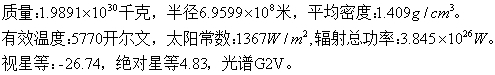
\includegraphics{const_sun.jpg}
\section{月球的基本数据}
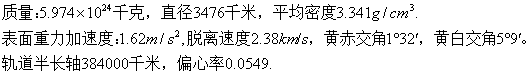
\includegraphics{const_moon.png}
\section{地球的基本数据}
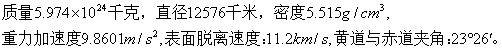
\includegraphics{const_earth.png}
\section{全天亮星}
\begin{center}
	\begin{tabular}{|l|l|l|l|l|l|l|}
		\hline
		亮度排名 & 星座英文名 & 英文名 & 视星等 & 距离(光年) & 中文名 & 所属星座 \\ \hline
		1 & Canis Major & Sirius & -1.46 & 8.6 & 天狼星 & 大犬座 \\ \hline
		2   & Canopus & Carina & -0.72  & 80 & 老人星 & 船底座 \\ \hline
		3 & Centaurus & Rigil Kent  & -0.27 & 4.3 & 南门二 & 半人马座 \\ \hline
		4 & Arcturus & Bootes & - 0.04 & 30 & 大角 & 牧夫座 \\ \hline
		5 & Vega & Lyra & +0.03 & 25 & 织女一 & 天琴座 \\ \hline
		6 & Capella & Ariga & +0.08 & 40 & 五车二 & 御夫座 \\ \hline
		7 & Rigel & Orion & +0.12 & 700 & 参宿七 & 猎户座 \\ \hline
		8 & Procyon & Canis Minor & +0.38 & 11 & 南河三 & 小犬座 \\ \hline
		9 & Achernar & Eridanus & +0.46 & 80 & 水委一 & 波江座 \\ \hline
		10 & Betelgeuse & Orion & +0.50 & 500 & 参宿四 & 猎户座 \\ \hline
		11 & Hadar & Centaurus & +0.61 & 330 & 马腹一 & 半人马座 \\ \hline
		12 & Altair & Aquila & +0.77 & 16 & 河鼓二 & 天鹰座 \\ \hline
		13 & Acrux & Crux & +0.87 & 350 & 十字架二 & 南十字座 \\ \hline
		14 & Antares & Scorpius & +0.96 & 500 & 心宿二 & 天蝎座 \\ \hline
		15 & Spica & Virgo & +0.98 & 350 & 角宿一 & 室女座 \\ \hline
		16 & Pollux & Gemini & +1.14 & 35 & 北河三 & 双子座 \\ \hline
		17 & Fomalhaut & Piscis Austrinus & +1.16 & 22 & 北落师门 & 南鱼座 \\ \hline
		18 & Deneb & Cygnus & 1.25 & 1800 & 天津四 &天鹅座\\ \hline
		19 & Mimosa & Crux & 1.25 & 500 & 十字架三 &南十字座\\ \hline
		20 & Regulus & Leo & 1.35 & 70 & 轩辕十四 &狮子座\\ \hline
		21 & Adhara & Canis Major & 1.5 & 600 & 弧矢七 &大犬座\\ \hline
	\end{tabular}
\end{center}
\section{天文常用的数学和物理常数}
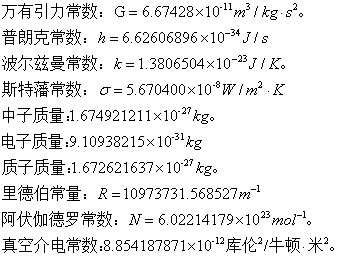
\includegraphics{const1.png}

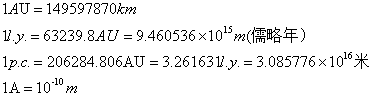
\includegraphics{const2.png}

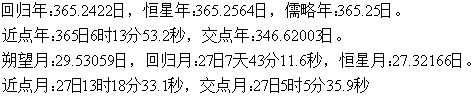
\includegraphics{const3.png}
\section{天文常数系统}
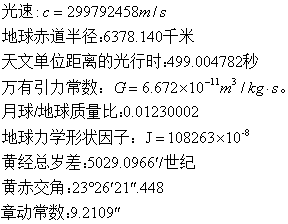
\includegraphics{const6.png}

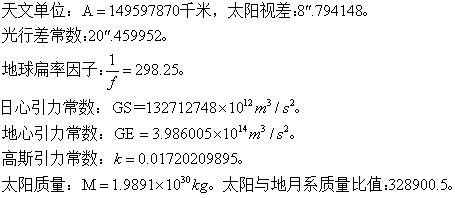
\includegraphics{const5.png}
\section{银河系基本情况}
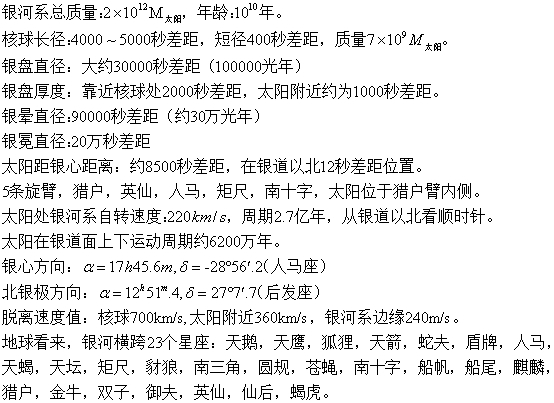
\includegraphics{const_milky_way.jpg}

\section{其他常用的数据}
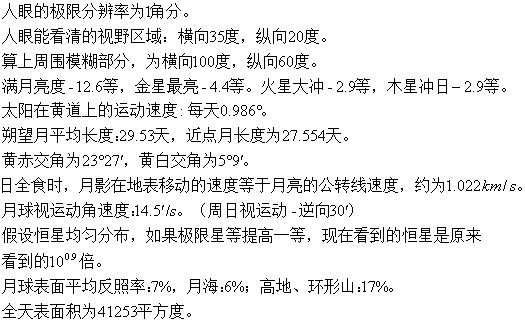
\includegraphics[scale=1.1]{const4.png}
\section{全天88星座列表}
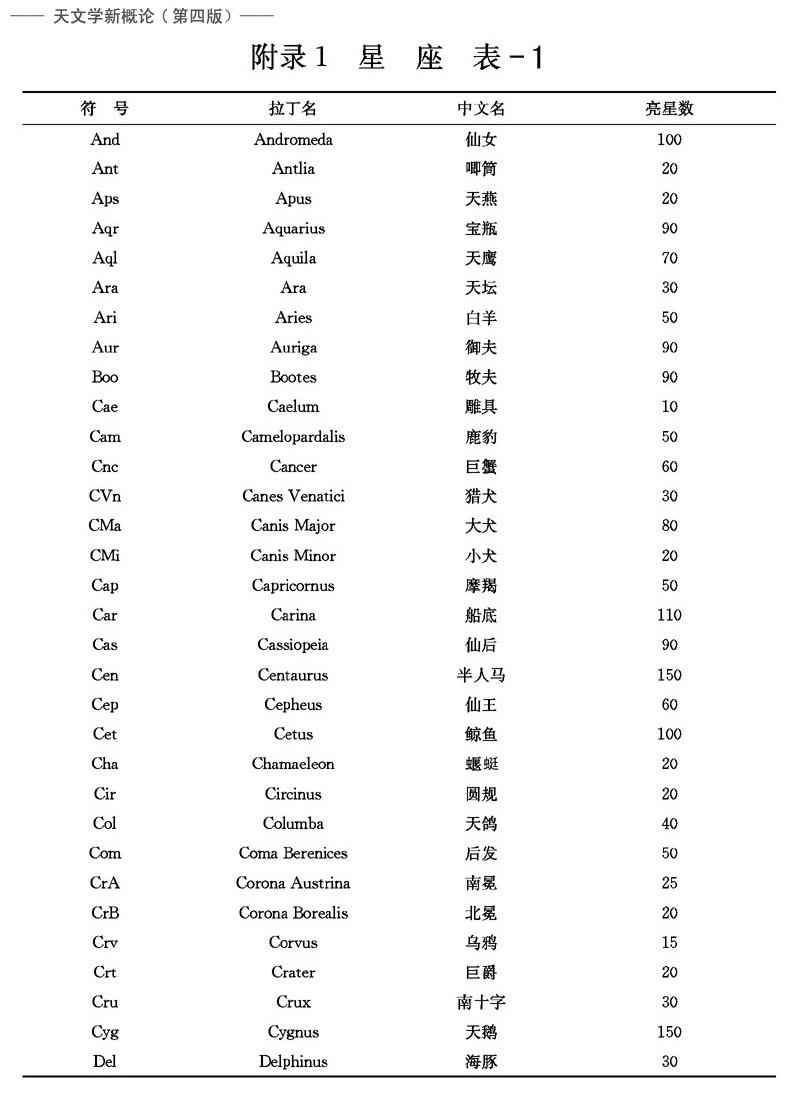
\includegraphics[scale=0.55]{Const_A.jpg}

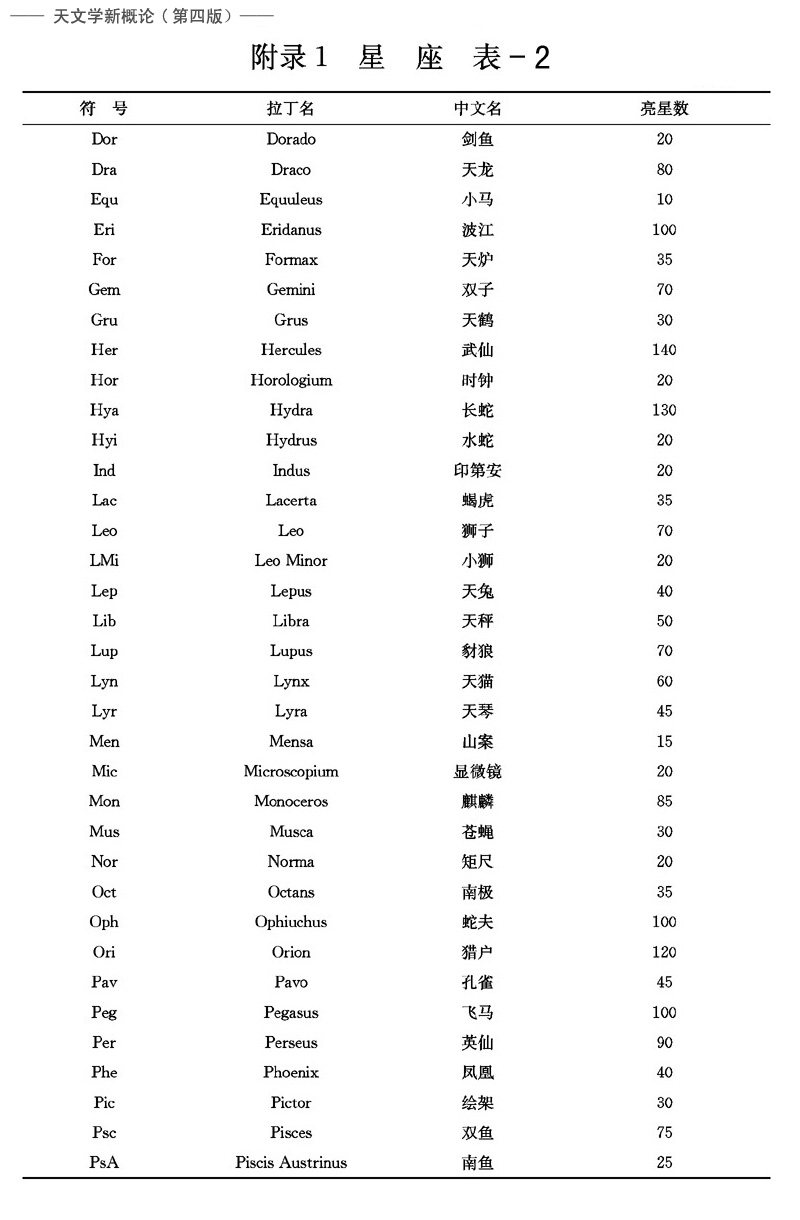
\includegraphics[scale=0.55]{Const_B.jpg}

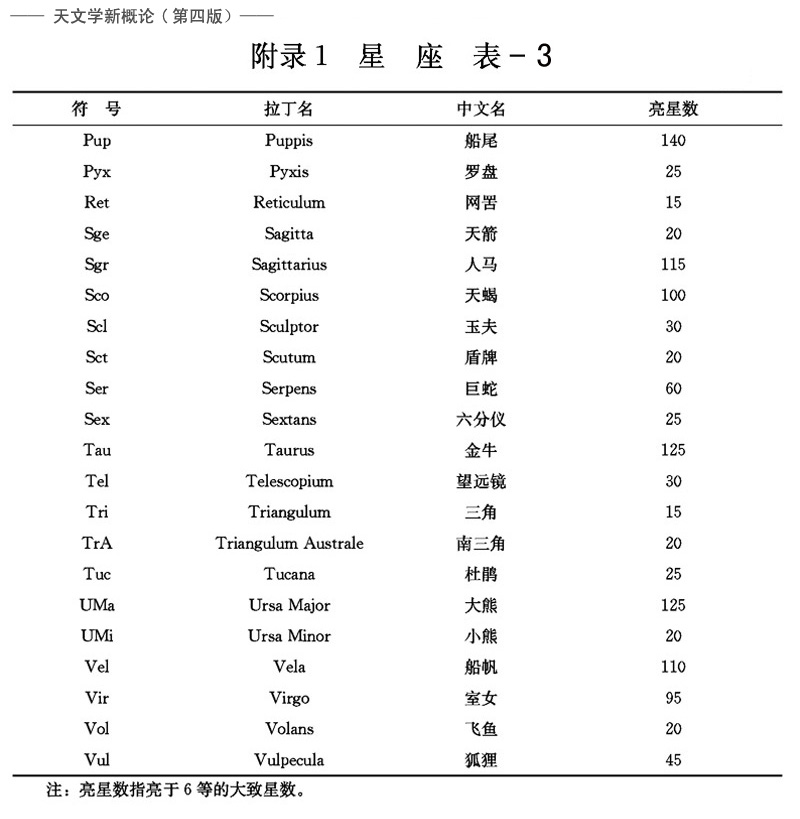
\includegraphics[scale=0.55]{Const_C.jpg}
\section{梅西叶星表}
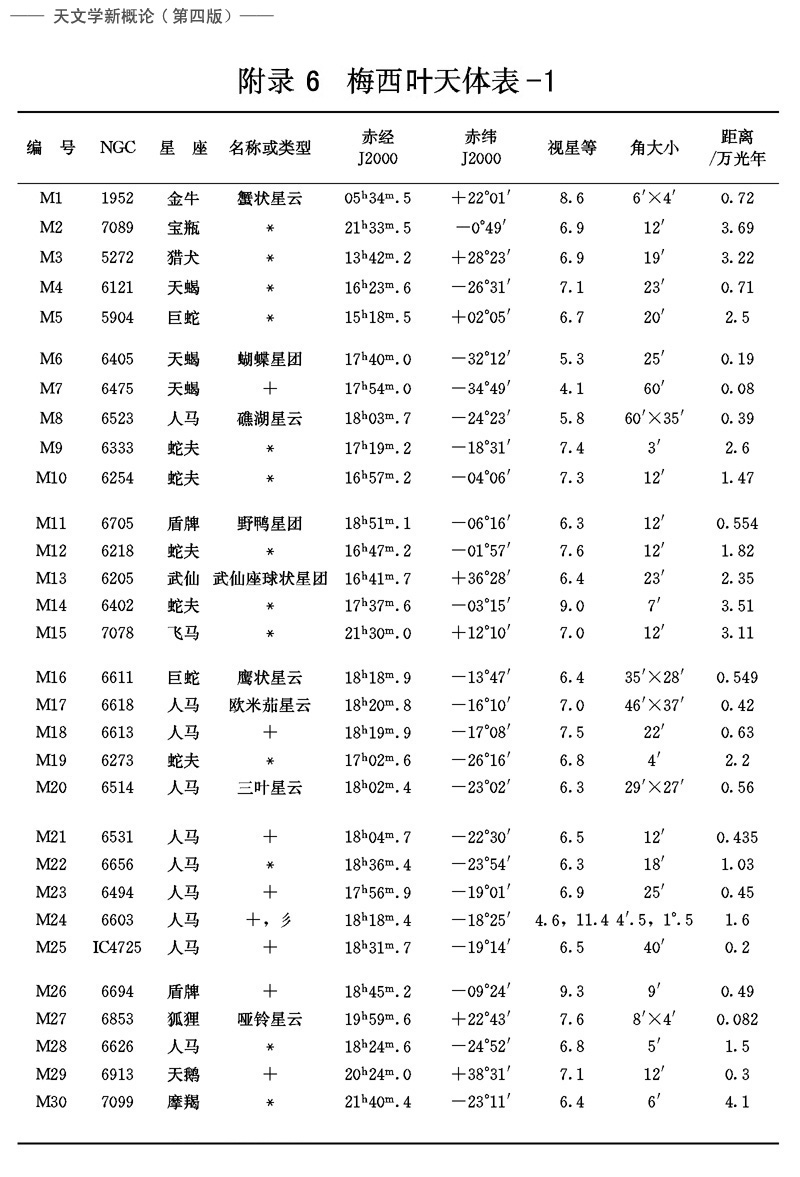
\includegraphics[scale=0.55]{messier_1.jpg}

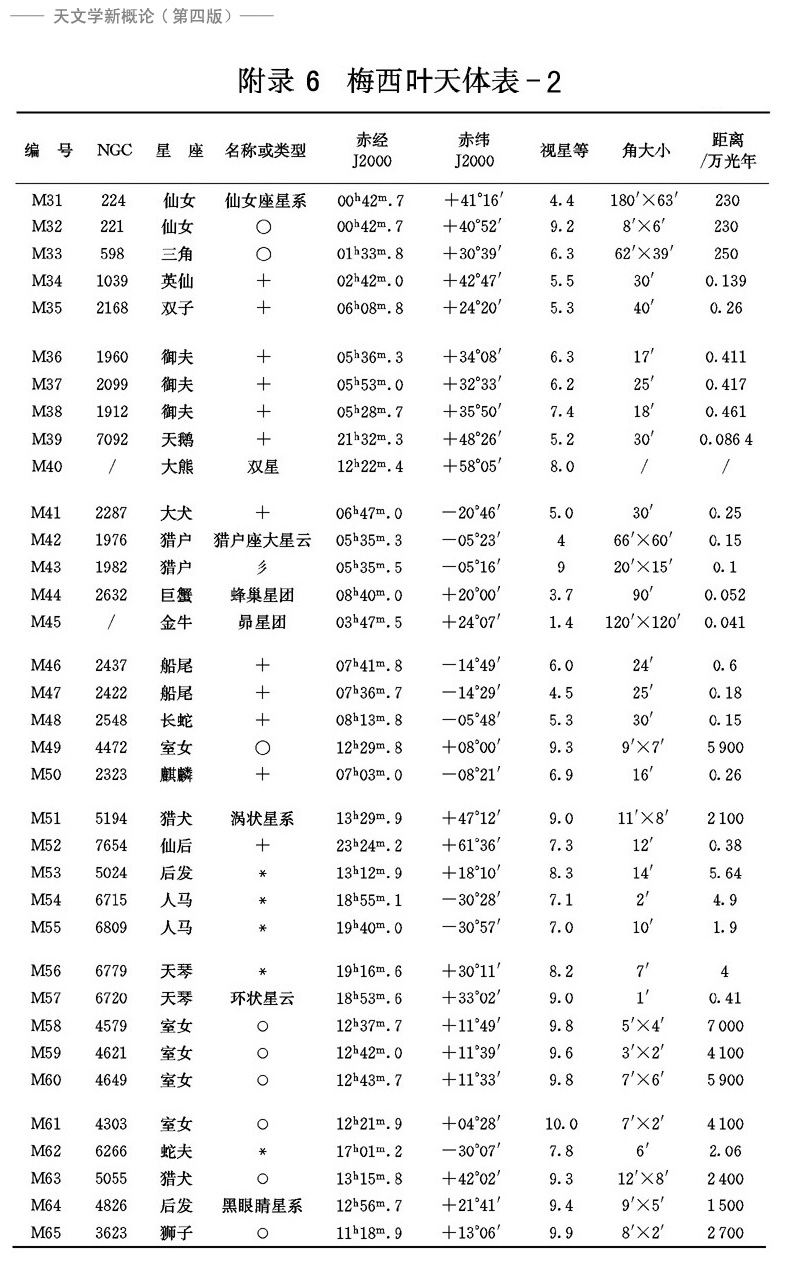
\includegraphics[scale=0.55]{messier_2.jpg}

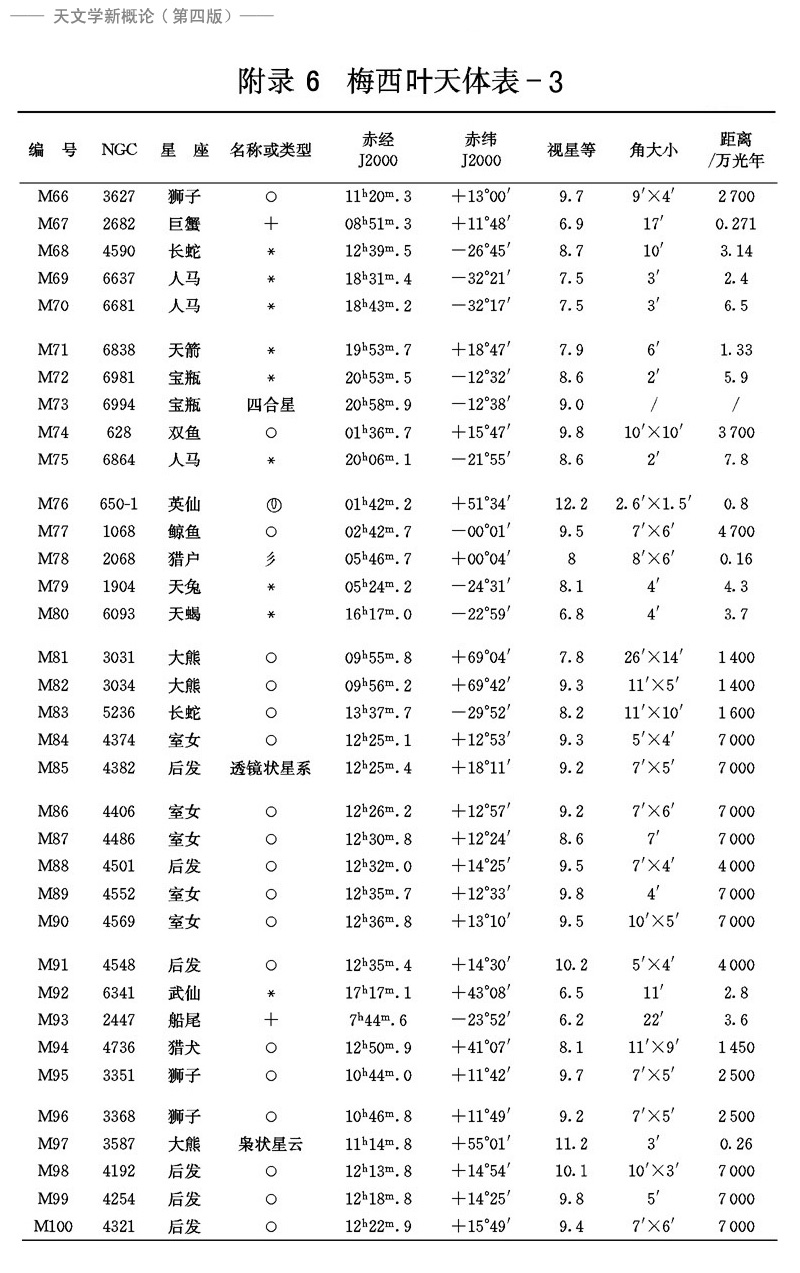
\includegraphics[scale=0.55]{messier_3.jpg}

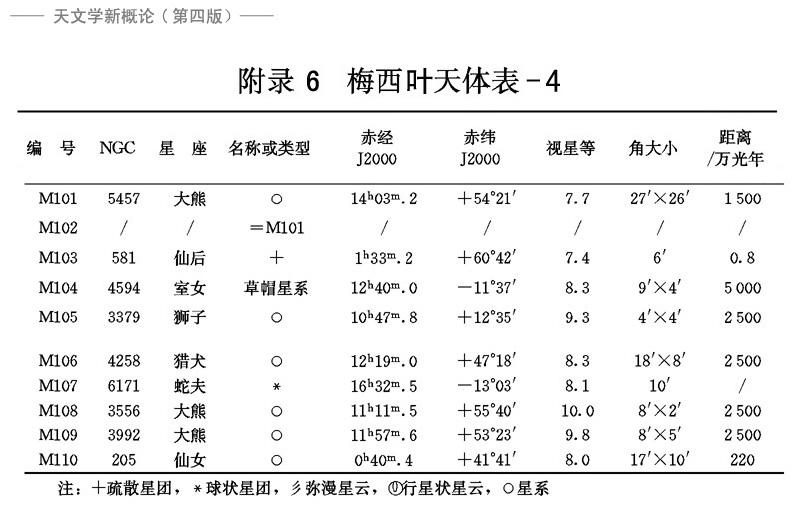
\includegraphics[scale=0.55]{messier_4.jpg}
\section{本星系群某些成员的部分参数}
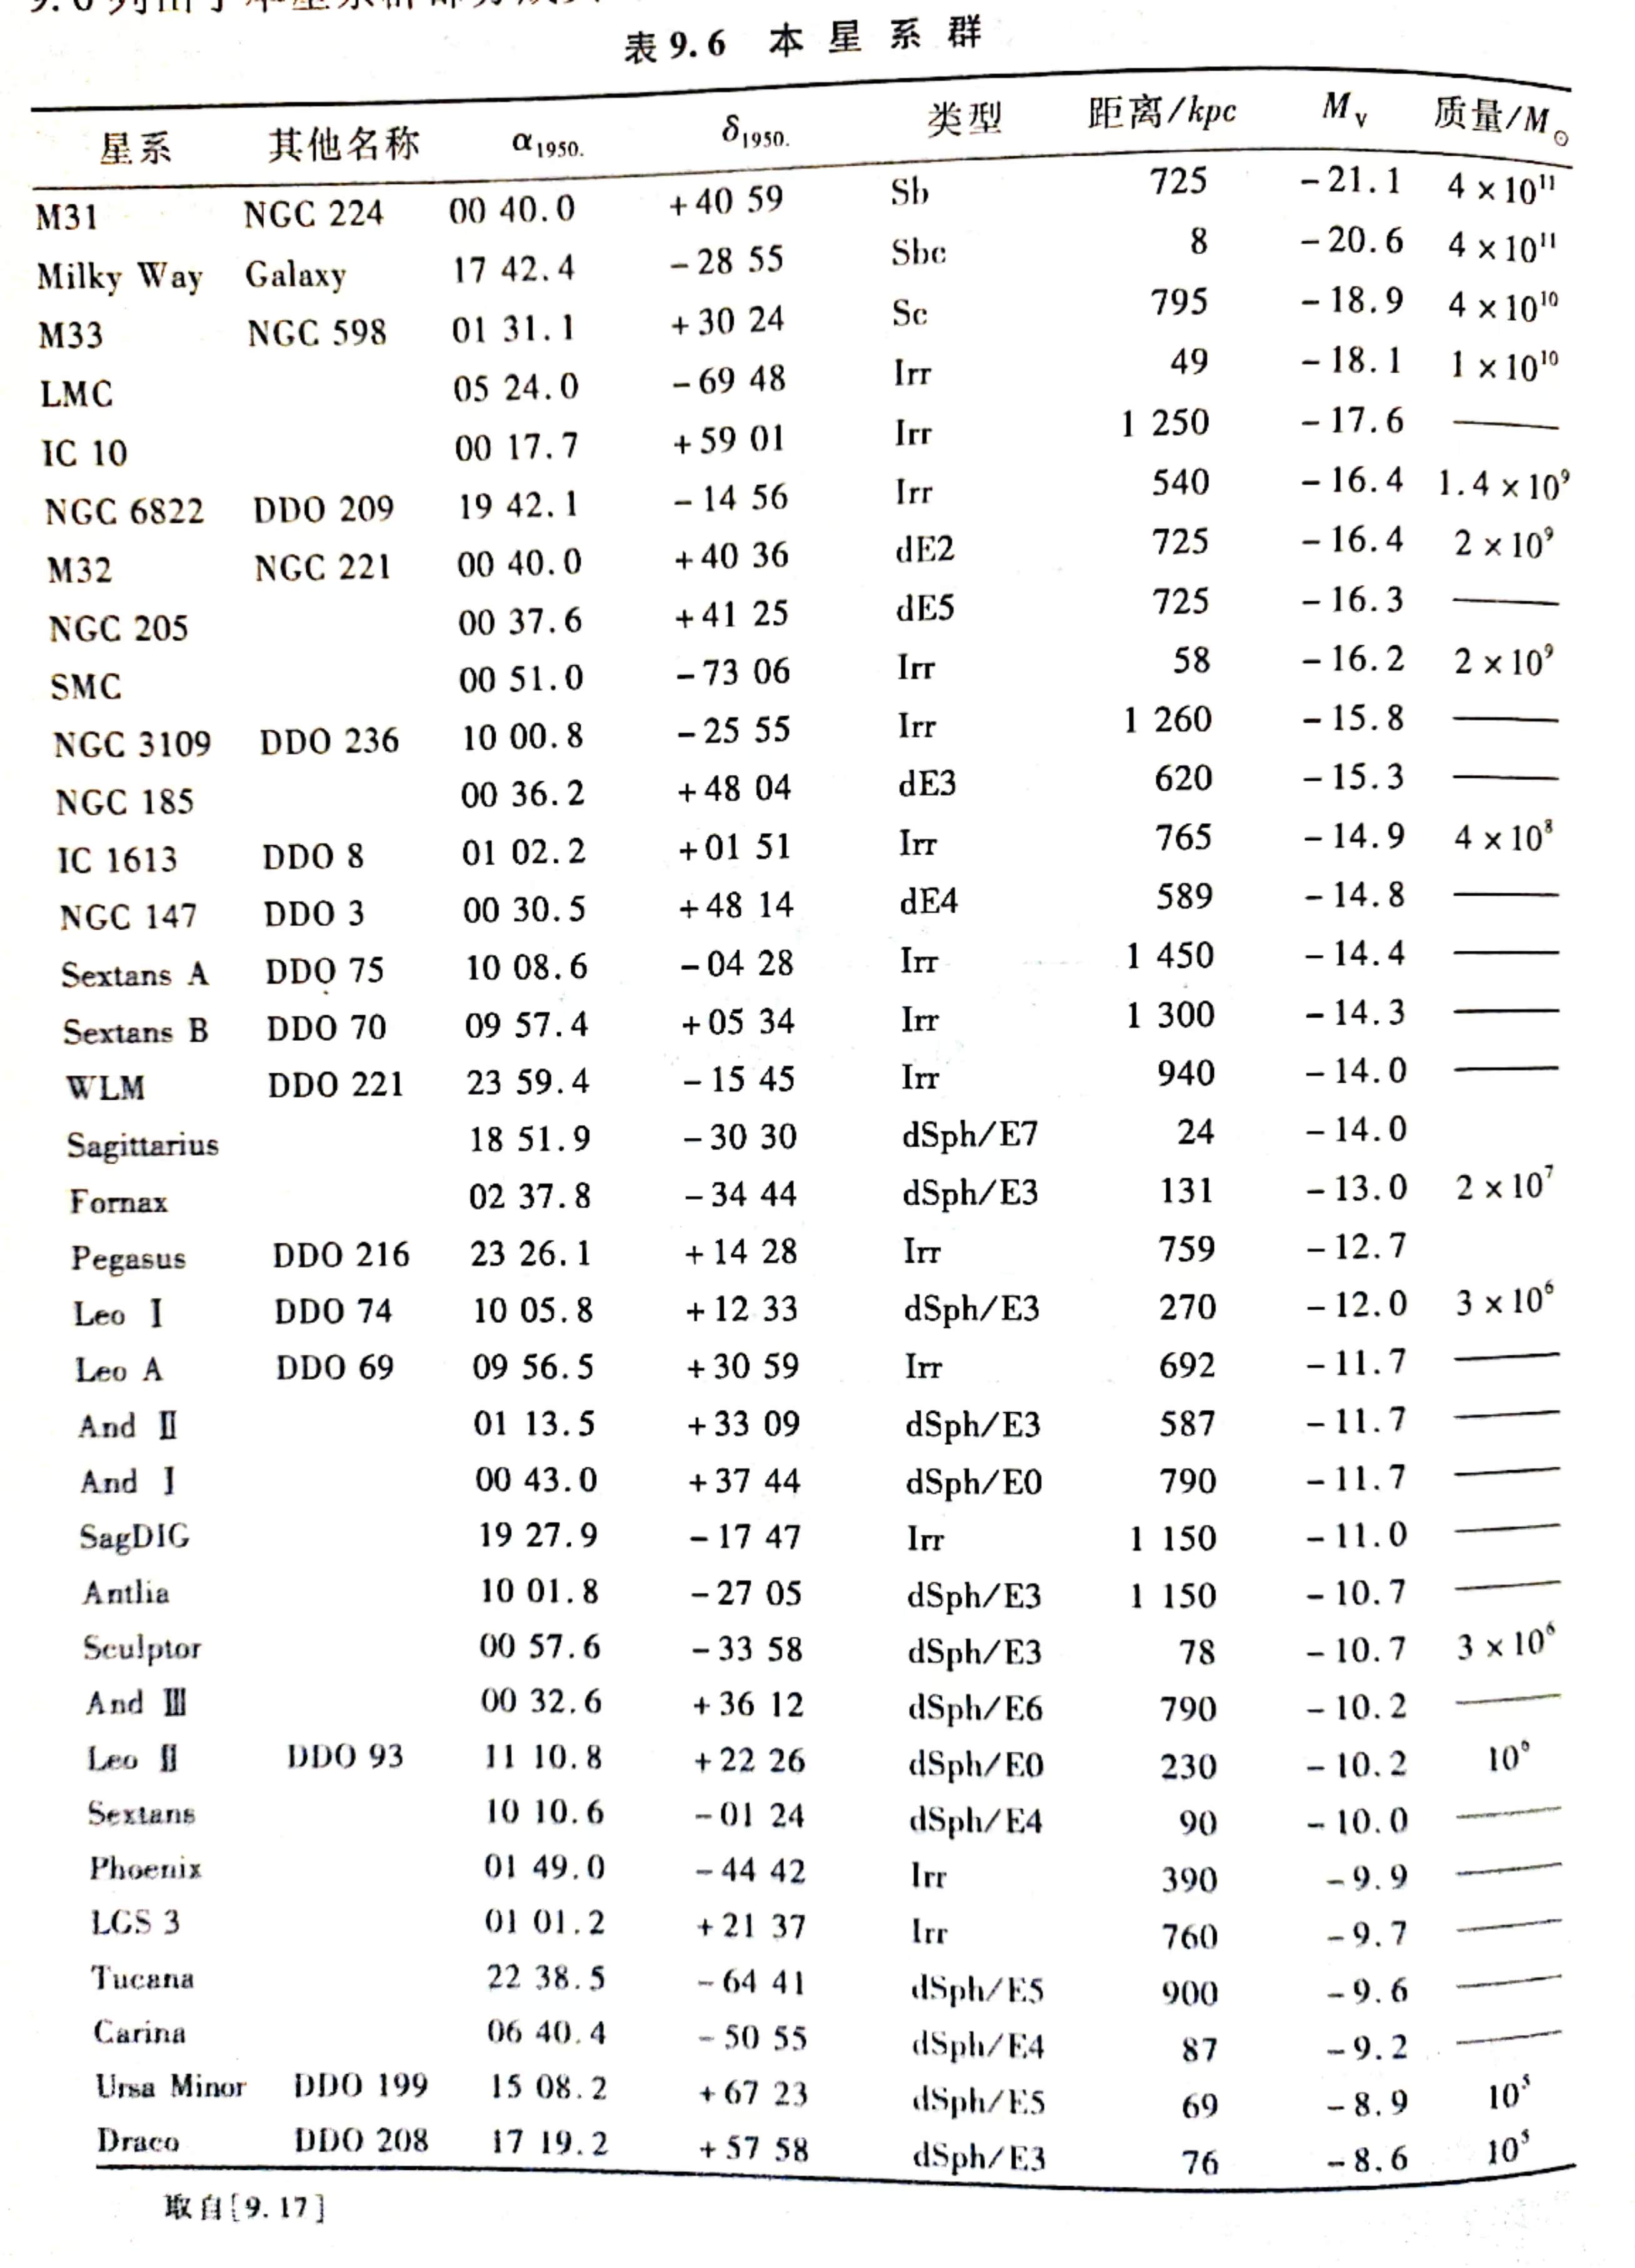
\includegraphics[scale=0.16]{bxxq.jpg }
\section{距离太阳最近恒星的物理参数}
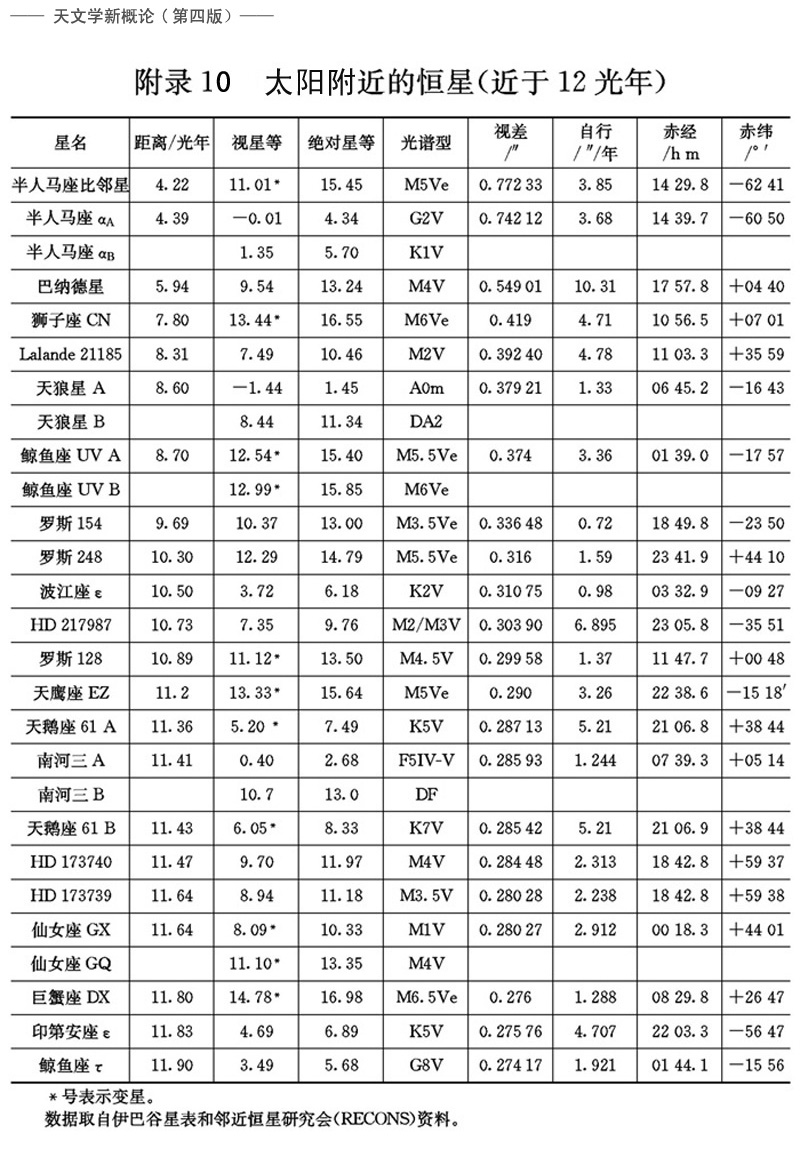
\includegraphics[scale=0.55]{zjhx.jpg}
\section{部分亮星的中国古代星名}
	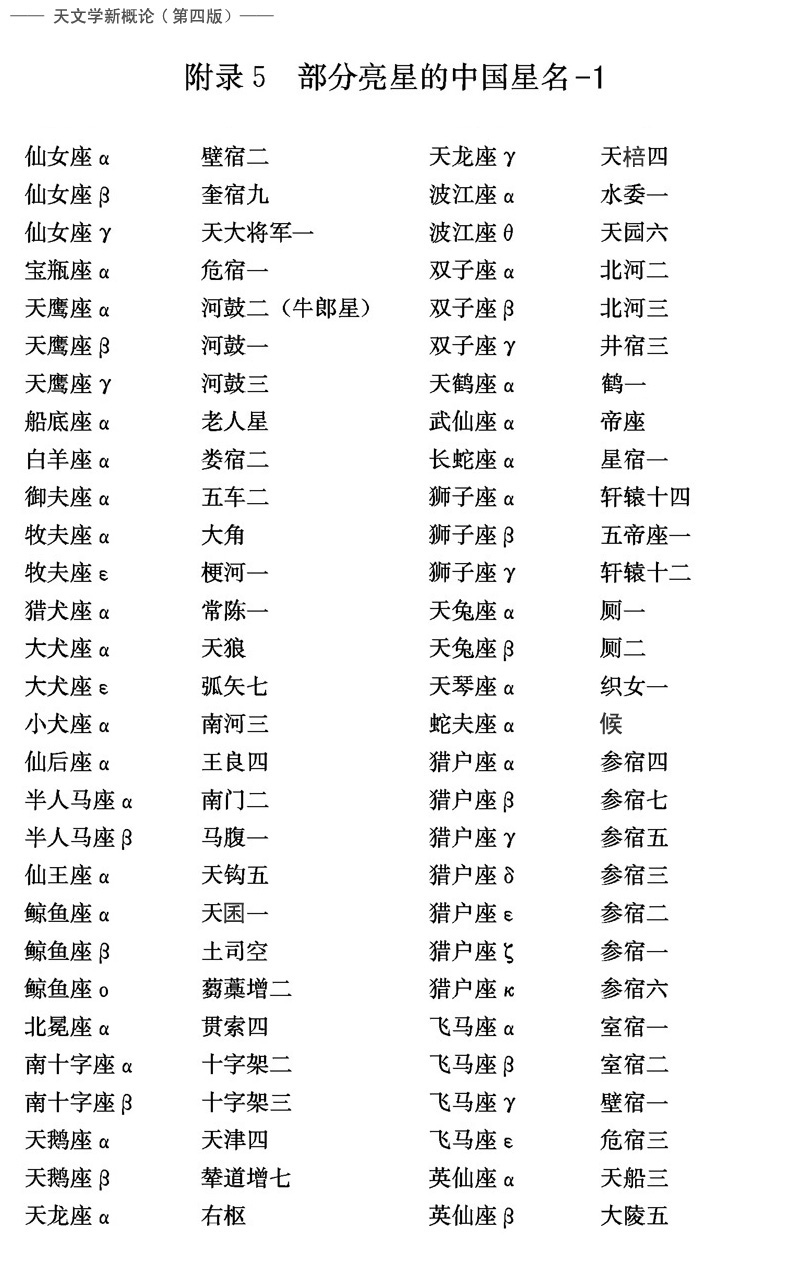
\includegraphics[scale=0.5]{ancient_1.jpg}
	
	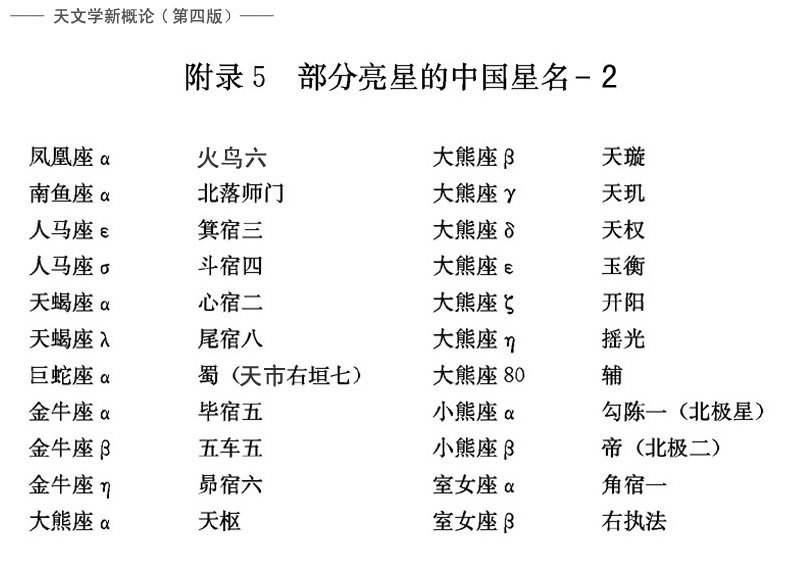
\includegraphics[scale=0.55]{ancient_2.jpg}
\chapter{参考文献}
刘学富《基础天文学》

苏宜《天文学新概论(第四版)》

肖兴华,李宗伟《天体物理学(第二版)》

《SSAA天文探索》

李光宇《天体测量与天体力学基础》

《天文爱好者》杂志2010增刊《天文奥赛指南》

《诺顿星图手册》

何香涛《观测宇宙学(第二版)》

向守平《天体物理概论》

《天文爱好者》2016年一月至2018年3月所有杂志。

本文档插入的图片中,除以下内容外,均取自苏宜《天文学新概论》第四版的光盘图附录:

本星系群某些成员的部分参数,取自《天体物理学》第二版第418页。

太阳、月球、地球的基本数据,天文常数系统,天文常用的数学和物理常数,银河系基本情况,其他常用的数据:
直接来源是第十五版复习资料的附录部分,根本来源是《天文学新概论》第四版的附录部分。